\documentclass[12pt]{article}
\usepackage{xr-hyper}
\externaldocument{supplement}
\usepackage{hyperref}
\usepackage[english]{babel}
\usepackage{graphicx}
\usepackage{framed}
\usepackage[normalem]{ulem}
\usepackage{amsmath}
\usepackage{amsthm}
\usepackage{amssymb}
\usepackage{amsfonts}
\usepackage{enumerate}
\usepackage{graphicx} % Allows including image
\usepackage{mathtools}
\hypersetup{
  linkcolor  = blue,
  citecolor  = blue,
  urlcolor   = blue,
  colorlinks = true,
} % color setup
\usepackage[utf8]{inputenc}
\usepackage[margin=1in]{geometry}
\usepackage{float} % for "H" placement specifier
\usepackage[authoryear]{natbib}
\usepackage{indentfirst}
\usepackage[dvipsnames]{xcolor}
\usepackage{array}
\usepackage{subcaption}
\usepackage{caption}
\usepackage[T1]{fontenc}
\usepackage{tikz}
\newcommand{\fatterdot}{\raisebox{0.15ex}{\tikz\filldraw[black,x=1.5pt,y=1.5pt] (0,0) circle (1);}}
\newcommand{\xn}{x^{\frac{1}{n}}}
\newcommand{\xnone}{x^{\frac{1}{n+1}}}

\newcommand{\R}{\mathbb{R}}
\DeclareUnicodeCharacter{FB01}{fi}
\DeclareUnicodeCharacter{FF0C}{,}
\DeclareMathOperator*{\Prob}{P}
\DeclareMathOperator*{\argmax}{arg\,max}
\DeclareMathOperator*{\argmin}{arg\,min}
\setlength\extrarowheight{1pt}

\newcommand\red[1]{{\color{red}#1}}

\bibliographystyle{plainnat}

\newtheorem{theorem}{Theorem}[section]
\newtheorem{corollary}{Corollary}[theorem]
\newtheorem{lemma}[theorem]{Lemma}
\newtheorem{prop}[theorem]{Proposition}
\newtheorem{defn}[theorem]{Definition}
\allowdisplaybreaks

\usepackage{setspace}
\doublespacing

\title{A Formal Investigation of Paradoxes Between Latent Aptitude and Observed Achievement via Full House Methodology}
\author{Daniel J. Eck$^1$, Shen Yan$^1$\thanks{email addresses: Daniel J. Eck (\url{dje13@illinois.edu});  Shen Yan (\url{shenyan3@illinois.edu})}}

\date{}

\begin{document}

\maketitle

{\centering
1. Department of Statistics, University of Illinois Urbana-Champaign \\}


\begin{abstract}
We study a paradox in which an individual with greater latent aptitude exhibits lower observed achievement than an individual with lesser aptitude when comparisons are made across contexts. We formalize this phenomenon as the aptitude-achievement paradox and introduce its probability as an explicit inferential target. To study this quantity, we employ Full House Modeling, a framework that derives latent aptitude from observed achievement by embedding observed samples within larger source populations. We derive closed-form paradox probabilities when achievement distributions are identical across contexts and obtain explicit expressions and bounds when they differ, including tractable results under normality with reliable plug-in estimation. Our results show that paradox risk depends primarily on population and sampling ratios rather than absolute sizes. An application to Major League Baseball contextualizes historically extreme batting performances, showing how modern achievements may appear less exceptional after accounting for population depth and measurement environments. By elevating aptitude-achievement reversals from anecdotal concern to an estimable quantity, this work provides a formal framework for quantifying structural reversals in cross-context comparisons under explicit models of population depth, selection, and measurement.
\end{abstract}


\subsection*{Highest-Priority Revision Checklist for JRSS-B Submission}

These revisions are aimed at improving both:
\begin{enumerate}
    \item overall fit with the stated JRSS-B scope, and
    \item reviewer perception of contribution density and methodological importance.
\end{enumerate}

\subsubsection*{Tier 1: Highest Priority Revisions}
\begin{enumerate}
    \item \textbf{Compress the application sections.}
    \begin{itemize}
        \item Retain only the most compelling illustrations of:
        \begin{itemize}
            \item paradox probabilities,
            \item latent-observed reversals,
            \item and empirical interpretability.
        \end{itemize}
    \end{itemize}
\end{enumerate}

\subsubsection*{Tier 2: Important Revisions}

\begin{enumerate}
    \item \textbf{Sharpen the inferential framing in Section 4.}
    \begin{itemize}
        \item Emphasize:
        \begin{itemize}
            \item computational tractability,
            \item operational estimation,
            \item and practical implementation.
        \end{itemize}
    \end{itemize}

    \item \textbf{Tighten the asymptotic rigor in Theorem 4.5.}
    \begin{itemize}
        \item Reduce heuristic EVT-style arguments where possible.
    \end{itemize}

    \item \textbf{Reduce defensive discussion of assumptions.}
    \begin{itemize}
        \item Shorten repeated caveats regarding:
        \begin{itemize}
            \item rank preservation,
            \item idealization,
            \item and selection assumptions.
        \end{itemize}
        \item Replace apologetic framing with concise scope clarification.
    \end{itemize}

    \item \textbf{Remove or reduce conjectural discussion.}
    \begin{itemize}
        \item In particular, consider moving the conjecture following Proposition~3.5 to the Discussion or Supplementary Materials.
    \end{itemize}
\end{enumerate}

\subsubsection*{Tier 3: Secondary but Valuable Revisions}

\begin{enumerate}
    \item \textbf{Shorten the Discussion section considerably.}
    \begin{itemize}
        \item Avoid re-running the Introduction.
        \item Focus on:
        \begin{itemize}
            \item broader methodological implications,
            \item selective observation,
            \item and future directions.
        \end{itemize}
    \end{itemize}

    \item \textbf{Reduce repeated philosophical exposition.}
    \begin{itemize}
        \item Compress repeated conceptual discussion of:
        \begin{itemize}
            \item aptitude vs.\ achievement,
            \item population depth,
            \item and contextual comparison.
        \end{itemize}
    \end{itemize}

    \item \textbf{Potentially revise the title toward a more methodological/statistical foundations framing.}
    \begin{itemize}
        \item Current title emphasizes ``paradoxes'' and may sound overly conceptual.
        \item Consider framing around:
        \begin{itemize}
            \item selective observation,
            \item latent-observed ranking reversals,
            \item or comparative inference.
        \end{itemize}
    \end{itemize}
\end{enumerate}



\section{Introduction}

Comparisons of outcomes across differing contexts, schools, regions, eras, institutions, and tasks are central to education and psychometrics \citep{holland2012differential, bond2013applying}, labor economics \citep{nickell1999labor}, medicine, and sports analytics \citep{BRL99, SM13, SM16, winston2022mathletics, yan2025comparing}. These problems have led to the development of a variety of widely used modeling frameworks that estimate relative ability, including empirical-Bayes shrinkage \citep{efron1975data}, Bayesian hierarchical models \citep{raudenbush1986hierarchical, BRL99}, Bradley-Terry-Luce and paired comparisons models \citep{bradley1952rank, bradley1976science, bradley1984paired, david1988paired}, Elo-type dynamic rating systems \citep{elo1978rating, graepel2007bayesian}, Gaussian-process and state-space formulations \citep{chu2005gaussian, houlsby2012collaborative}, item-response and latent class models \citep{mcdonald1999test, embretson2000item, hagenaars2002applied, holland2012differential, bond2013applying}, factor models \citep{mcdonald1999test, bartholomew2011latent}, and domain-specific metrics \citep{baumer2014statistician, BB15, yu2016pantheon}.

Despite their differences, these approaches share a common structural feature: ability is inferred relative to a fixed or implicitly comparable set of observed competitors. While such models adjust outcomes within a given context, they do not typically explicitly account for changes in the size or structure of the eligible population, nor for context-specific distortions in how latent ability is expressed through observed outcomes. Consequently, when competition depth, selection mechanisms, or measurement conditions vary across contexts, observed dominance may not reliably reflect the corresponding latent ordering.

These limitations give rise to a new inferential target: the probability that cross-context comparisons reverse latent aptitude orderings. Specifically, an individual drawn from a deeper or more competitive population may possess higher latent aptitude yet exhibit lower observed achievement than a counterpart from a shallower or more weakly filtered context. We term this phenomenon the aptitude-achievement paradox. Formally, let individual $j$ in context $i$ have observed $\mathbb{R}$-valued achievement $Y_{i,j}$ and latent $\mathbb{R}$-valued aptitude $X_{i,j}$, and let individual $n$ in context $m$ have observed achievement $Y_{m,n}$ and latent aptitude $X_{m,n}$. The probability of an aptitude-achievement paradox is
\begin{equation} \label{eq:paradoxgeneral}
	\Prob\left(X_{i,j} > X_{m,n}, Y_{i,j} < Y_{m,n}\right).
\end{equation}
This quantity captures the structural risk that comparisons based on observed outcomes reverse the corresponding latent ordering across contexts.

Such reversals arise naturally when measurement systems differ across contexts or when observation occurs through non-random selection mechanisms shaped by institutional, competitive, or environmental constraints. Existing methods provide limited tools for quantifying the frequency of these reversals.

Related work has studied disagreement between observed rankings and target orderings through measures such as Kendall's $\tau$ \citep{kendall1938new} and Somers' $D$ \citep{somers1962new}, while latent-trait and comparative ability models---including Rasch models \citep{bond2013applying}, Bayesian hierarchical formulations \citep{raudenbush1986hierarchical, BRL99}, and Elo-type rating systems \citep{elo1978rating, graepel2007bayesian}---infer underlying ability from observed outcomes. However, these approaches generally operate relative to the observed comparison pool and do not explicitly model how differences in eligible population depth, selection intensity, or measurement environments distort the relationship between latent aptitude and observed achievement.

To address these limitations, we develop a structural framework for cross-context comparison that explicitly models population depth, selective observation, and context-specific measurement processes. This framework, which we refer to as Full House Modeling (FHM), was initially proposed in an applied setting comparing baseball players across eras \citep{yan2025comparing}, and is formalized here for comparative analysis across heterogeneous contexts. Under FHM, individuals are drawn from a common latent aptitude distribution, while contexts differ in (i) the size of the eligible population, (ii) the mechanism through which individuals are selected into observation, and (iii) the mapping from latent aptitude to observed achievement. We model measurement through context-specific rank-preserving transformations between latent aptitude and observed achievement.

In this paper, we develop the theory of FHM under rank-based selection mechanisms, particularly top-$n$ selection, where tractable results are available. These assumptions are most natural in highly selective settings where observed individuals represent the upper tail of a larger latent population. Comparisons of athletes across eras provide a canonical example, since entry into professional leagues closely approximates selection of the most talented individuals from large underlying populations.

\citet{yan2025comparing} introduced Full House Modeling as an operational methodology for cross-era comparison in baseball analytics. The present paper develops the first formal statistical theory for this framework. In particular, our contributions are as follows:
\begin{itemize}
    \item We formalize the aptitude-achievement paradox as an explicit inferential target for cross-context comparison and study its probability under selective observation.
    \item We develop the probabilistic foundations of Full House Modeling, including a characterization result showing that the induced latent-observed coupling is the unique rank-preserving monotone transformation consistent with the model assumptions.
    \item Under identical observed achievement distributions across contexts, we derive explicit and distribution-free paradox probabilities and characterize their dependence on population and sampling structure.
    \item Under heterogeneous achievement distributions, we derive general bounds and obtain tractable asymptotic approximations in Gaussian settings, including explicit remainder bounds and plug-in consistency results.
    \item We show through theoretical analysis and sensitivity experiments that paradox probabilities depend primarily on ratios of eligible population sizes and sampling fractions rather than their absolute magnitudes.
\end{itemize}

Proofs of mathematical results are provided in the Supplementary Materials.


%A large class of methods studies disagreement between observed orderings and target rankings. Classic examples include Kendall's $\tau$ \citep{kendall1938new} and Somers' $D$ \citep{somers1962new}, which summarize concordance and discordance between observed rankings. However, these approaches operate entirely on observed outcomes and do not explicitly model latent aptitude, population depth, or selection into observation.

%Traditional latent trait models \citep{bartholomew2011latent} instead focus on estimating underlying ability from observed categorical or discrete outcomes. For example, the Rasch model \citep{bond2013applying} ensures that comparisons of individual abilities are invariant to the specific items administered under assumptions excluding differential item functioning (DIF) \citep{holland2012differential}. Likewise, Bayesian hierarchical and state-space models for latent ability---including Elo-type rating systems \citep{BRL99, elo1978rating, graepel2007bayesian}---typically condition on the observed competitive or testing pool and account for heterogeneity through random effects or temporal evolution, without explicitly modeling variation in eligible population depth or selection across contexts.


%These limitations give rise to a previously unquantified inferential target: the probability that cross-context comparisons reverse latent orderings. Specifically, an individual drawn from a deeper or more competitive population may possess higher latent aptitude yet exhibit lower observed achievement than a counterpart from a shallower or more weakly filtered context. We term this phenomenon the aptitude-achievement paradox. Formally, let individual $j$ in context $i$ have an observed $\R$-valued statistic $Y_{i,j}$ and an underlying latent $\R$-valued aptitude $X_{i,j}$, and let individual $n$ in context $m$ have an observed $\R$-valued statistic $Y_{m,n}$, and an underlying latent $\R$-valued aptitude $X_{m,n}$. The probability of aptitude-achievement paradox is 
%\begin{equation} \label{eq:paradoxgeneral}
%	\Prob\left(X_{i,j} > X_{m,n}, Y_{i,j} < Y_{m,n}\right) 
%\end{equation}
%This quantity captures the structural risk that cross-context comparisons based on observed outcomes reverse the true latent ordering.

%Such reversals cannot occur if aptitude is mapped to achievement through a common strictly increasing measurement mechanism and if selection into observation is ignorable. In practice, however, measurement systems often differ across contexts, and observed individuals are typically selected through non-random processes shaped by institutional, competitive, or environmental constraints. As a result, observed dominance may reflect differences in selection intensity or measurement conditions rather than differences in underlying aptitude. Existing methods provide limited tools for quantifying the frequency of such reversals under explicit models of aptitude, selection, and measurement.

%The aptitude-achievement paradox in Eq \ref{eq:paradoxgeneral} cannot arise if a single, strictly increasing, context-invariant measurement map relates aptitude to achievement and if selection into tasks is ignorable. In practice, however, both measurement heterogeneity (non-invariance, differential item functioning) and non-ignorable selection (who attempts which tasks, faces which opponents, receives which treatment) are pervasive. These features can reverse cross-context rankings even when the latent ranking is unambiguous, echoing classic reversal phenomena such as Simpson's \citep{simpson1951interpretation} and Lord's paradoxes \citep{lord1967paradox} while implicating modern concerns about fairness. What practitioners lack is a principled way to quantify how often such reversals should occur under an explicit model of aptitude, measurement, and selection.

%A large class of methods quantifies how often observed orderings disagree with a target ordering, closely related to the phenomenon studied here. Classic examples include rank-discordance measures such as Kendall's $\tau$ \citep{kendall1938new} and Somers' $D$ \citep{somers1962new}, which summarize the frequency of concordant and discordant pairs based on observed rankings. Because these indices operate entirely on observed outcomes, they neither place individuals on a common latent scale nor disentangle the effects of measurement non-invariance or selection, motivating models that make the measurement and selection processes explicit.

%Traditional latent trait models \citep{bartholomew2011latent} focus on estimating underlying abilities from observed categorical or discrete outcomes. For example, the Rasch model \citep{bond2013applying} ensures that comparisons of individuals' abilities are invariant to the specific items administered, under the assumption of no differential item functioning (DIF) \citep{holland2012differential}. However, such models do not explicitly leverage information about the size or structure of the source population from which individuals are drawn. Likewise, Bayesian hierarchical and state-space models for latent ability---including Elo-type rating systems \citep{BRL99, elo1978rating, graepel2007bayesian}---typically condition on the observed competitive or testing pool and capture population-level variation through random effects or dynamic evolution, without modeling variation in eligible population depth or selection into observation across contexts. In parallel, the causal bootstrap \citep{imbens2018causal} emphasizes that valid causal inference requires explicitly situating the observed sample within a larger source population, rather than treating the realized sample as the population of interest.


\section{Model Setting}
\label{sec:modelsetting}


We now motivate the structure of the Full House Model.  Let $N_i$ denote the size of population $i$. We distinguish between a \emph{population}, consisting of all individuals $N_i$ in context $i$, and a \emph{system}, which denotes the subset of individuals whose outcomes are observed or recorded. The system is determined by a selection mechanism that maps the full population into an observed sample of size $n_i$. We suppose that every individual $k = 1,\ldots, N_i$ has an underlying latent $\R$-valued aptitude $X_{i,1}, \ldots, X_{i,N_i} \overset{iid}{\sim} F_{X}$. Let $\textbf{X}_{i,-j}$ be the vector of all latent aptitudes not including the component $j$. We formalize the selection mechanism through an indicator function $S_{i,j} = 1_{i}\left(X_{i,j},\textbf{X}_{i,-j}\right)$, where $S_{i,j} = 1$ indicates inclusion in the observed system and a value of $S_{i,j} = 0$ indicates exclusion. This function may depend on the individual's aptitude relative to others in the population.

We now suppose that an individual $j$ included in system $i$ has an observed $\R$-valued statistic $Y_{i,j} \overset{iid}{\sim} F_{Y_i}$, $j = 1,\ldots,n_i$, with $n_i \leq N_i$. Under Full House Modeling, the observed values $Y_{i,j}$ are assumed to preserve the ranking induced by the latent aptitudes among the selected individuals.

Let $X_{i,(j)}$ and $Y_{i,(j)}$ denote the $j$th order statistic for system $i$. Here, larger values correspond to higher aptitude or achievement, so that $X_{i,(j)} > X_{i,(k)}$ whenever $j>k$. We form $(Y,X)$ pairs of random variables for each individual included in the system. These pairs are of the form $(Y_{i,(j)}, X_{i,(r_{i,j})})$, where $r_{i,j}$ indexes the rank of that individual's latent aptitude within the full population of size $N_i$.

As an example, consider the selection rule $S_{i,j} = 1 \;\Longleftrightarrow\; X_{i,j} \ge X_{i,(N_i-n_i+1)}$, which selects the top $n_i$ individuals in population $i$. In this case, the pairs take the form $(Y_{i,(j)}, X_{i,(N_i - n_i + j)})$ for $j = 1,\ldots,n_i$.

The key feature of Full House Modeling is the explicit connection between the elements forming the $(Y_{i,(j)}, X_{i,(r_{i,j})})$ pairs. This construction can be understood as a rank-preserving transformation between latent aptitude and observed achievement. Based on the probability integral transformation, Full House Modeling specifies this connection as
\begin{equation} \label{eq:truepar}
\begin{split}
  Y_{i, (j)} &= F_{Y_{i, (j)}}^{-1} \circ F_{X_{i, (r_{i,j})}} \left(X_{i, (r_{i,j})}\right), \\
  X_{i, (r_{i,j})} &= F_{X_{i, (r_{i,j})}}^{-1} \circ F_{Y_{i,(j)}} \left(Y_{i,(j)} \right),
\end{split}
\end{equation}
where $S_{i,j} = 1$, and both $F_{Y_i}$ and $F_X$ are continuous and invertible. We summarize Full House Modeling in the following definition.

\begin{defn} [Full House Model]
\label{def:fhm}
Consider populations indexed by $i$ with sizes $N_i$ and system sizes $n_i$, where $N_i \geq n_i$. Let latent variables $X_{i,j} \overset{iid}{\sim} F_X$, $j = 1,\ldots,N_i$, and define the selection indicators $S_{i,j} := 1_i(X_{i,j}, \mathbf{X}_{i,-j})$, where $S_{i,j}=1$ indicates inclusion in the observed system. Let $Y_{i,j} \overset{iid}{\sim} F_{Y_i}$, $j = 1,\ldots,n_i$, denote observed outcomes for the selected individuals. Form pairs $(Y_{i,(j)}, X_{i,(r_{i,j})})$, $j = 1,\ldots,n_i$, corresponding to the individuals for which $S_{i,j}=1$. Then the Full House Model generates $Y_{i,(j)}$ values according to \eqref{eq:truepar}, where $F_{Y_i}$ and $F_X$ are continuous and invertible.
\end{defn}

The Full House Model defines a joint distribution over $(X,Y)$ together with selection indicators $S_{i,j}$. Latent variables $X$ are drawn i.i.d.\ from $F_X$, and the selection indicators $S_{i,j}$ determine inclusion in the observed system. Conditional on inclusion, observed outcomes $Y$ are generated via a rank-preserving monotone coupling with $X$. In particular, the dependence between $X$ and $Y$ is induced through a quantile-matching transformation of their order statistics, ensuring that higher latent aptitude corresponds to higher observed achievement within each system. %The stochasticity in the Full House Model arises entirely from the latent population $X$, while both selection and observed outcomes are deterministic functionals of $X$.
Conditional on the latent population and the selection mechanism, observed outcomes are generated through a deterministic rank-preserving coupling.


The Full House Model induces structural missingness by construction: for any individual $j$ such that $S_{i,j} = 0$, the corresponding observed statistic $Y_{i,j}$ is undefined. In subsequent sections, we consider probabilities involving both latent and observed quantities. To formalize this setting, we treat $Y_{i,j}$ as a random variable defined only on the event $\{S_{i,j}=1\}$. For example, $\Prob\big(X_{i,j}\in A,\; Y_{i,j}\in B,\; S_{i,j} = 1\big)$ is well-defined for Borel sets \(A,B\subset \mathbb R\), whereas $Y_{i,j}$ is not defined on $\{S_{i,j} = 0\}$. This perspective allows selection mechanisms to be incorporated into probabilistic statements without imputing counterfactual outcomes.

Definition~\ref{def:fhm} assumes a common latent aptitude distribution $F_X$ across contexts, while allowing the observed achievement distributions $F_{Y_i}$ to vary by system. This reflects a modeling choice in which the process generating latent aptitude is taken to be context-neutral, whereas the expression and measurement of aptitude may differ across contexts.


Direct evaluation of the order-statistic distributions in \eqref{eq:truepar} is often cumbersome. However, under continuity, they admit a convenient representation in terms of Beta distributions. In particular,
\begin{equation} \label{eq:betarepX}
F_{X_{i,(r_{i,j})}}\!\left(X_{i,(r_{i,j})}\right)
= F_{U_{i,(r_{i,j})}} \circ F_X\!\left(X_{i,(r_{i,j})}\right),
\quad U_{i,(r_{i,j})} \sim \mathrm{Beta}\!\left(r_{i,j},\, N_i - r_{i,j} + 1\right),
\end{equation}
and similarly,
\begin{equation} \label{eq:betarepY}
F_{Y_{i,(j)}}\!\left(Y_{i,(j)}\right)
= F_{U_{i,(j)}} \circ F_{Y_i}\!\left(Y_{i,(j)}\right),
\quad U_{i,(j)} \sim \mathrm{Beta}\!\left(j,\, n_i - j + 1\right).
\end{equation}
This representation allows \eqref{eq:truepar} to be computed via $F_X$, $F_{Y_i}$, and known Beta distributions, bypassing explicit order-statistic calculations. It also implies that latent aptitude can be recovered up to a monotone transformation without explicit knowledge of $F_X$.

Combining \eqref{eq:betarepX} and \eqref{eq:betarepY} yields
$$
X_{i,(r_{i,j})} = F_X^{-1}\!\left(
F_{U_{i,(r_{i,j})}} \circ F_{U_{i,(j)}} \circ F_{Y_i}\!\left(Y_{i,(j)}\right)
\right).
$$
Define $W_{i,j} = F_{U_{i,(r_{i,j})}} \circ F_{U_{i,(j)}} \circ F_{Y_i}(Y_{i,(j)})$. Since $F_X$ is monotone, so is its inverse, which implies
$$
W_{i_1,j_1} \ge W_{i_2,j_2} \;\;\Longrightarrow\;\; 
F_X^{-1}(W_{i_1,j_1}) \ge F_X^{-1}(W_{i_2,j_2}).
$$
Thus the ordering of latent aptitudes is invariant to $F_X$, and $F_X$ acts as a structural nuisance parameter for comparative analysis. In practice, Full House Modeling can therefore be implemented via observed-to-rank mappings without requiring explicit specification of the latent distribution.

The representation in \eqref{eq:truepar} may appear as a modeling choice. The following result shows that, under natural invariance and rank-based assumptions, this construction is in fact essentially unavoidable.

\begin{theorem}[Characterization of Full House Coupling]
\label{thm:FHM-characterization-clean}
Fix a population $i$. Let $X_{i,1},\dots,X_{i,N_i}$ be i.i.d.\ from a continuous distribution $F_X$. Suppose there exists a set $\mathcal{R}_i \subset \{1,\dots,N_i\}$ such that $S_{i,j} = 1 \;\Longleftrightarrow\; r_{i,j} \in \mathcal{R}_i$, where $r_{i,j}$ is the rank of $X_{i,j}$ among $(X_{i,1},\dots,X_{i,N_i})$. 

For each observed rank $j$, suppose there exists a measurable strictly increasing function $\psi_{i,j}:\mathbb{R}\to\mathbb{R}$ such that $Y_{i,(j)} = \psi_{i,j}\!\big(X_{i,(r_{i,j})}\big)$ a.s., and assume $F_{Y_{i,(j)}}$ is continuous. Then, for each observed rank $j$,
$$
Y_{i,(j)} = F_{Y_{i,(j)}}^{-1} \circ F_{X_{i,(r_{i,j})}}\!\left(X_{i,(r_{i,j})}\right)
\quad \text{a.s.}
$$
Moreover, this representation is unique up to null sets and coincides with that induced by the Full House Model in Definition~\ref{def:fhm}.
\end{theorem}

\subsection{Interpretation and scope of the rank-preserving assumption}

The coupling in Definition~\ref{def:fhm} is intentionally structural rather than measurement-error based. Under Full House Modeling, observed outcomes are generated through a rank-preserving transformation of latent aptitude among selected individuals, so that stochasticity enters through the latent population and the selection mechanism rather than through additive observational noise. The framework is not intended as a literal noiseless measurement model. Rather, the framework is intended as an idealized abstraction of settings in which observed rankings primarily reflect latent ordering after strong selection into the observed system.

This abstraction is most plausible in highly selective environments, where observed individuals represent the upper tail of a much larger latent population and observed outcomes are designed to discriminate among top performers. Professional sports provide a canonical example: although season-level outcomes contain substantial variability, long-run elite performance is strongly constrained by selection into the league itself. In such settings, rank-preserving approximations provide a tractable framework for studying how population depth and selection interact with observed achievement.

More generally, Full House Modeling should be viewed as a structural model for latent-observed comparison under selective observation, rather than as a literal generative model for noisy repeated measurements. Extending the framework to incorporate stochastic measurement error, imperfect ranking preservation, or probabilistic selection mechanisms is an important direction for future work.


\section{Paradoxes Under Identical Achievement Distributions}
\label{sec:samedist}

In this section, we derive explicit probabilities of the aptitude--achievement paradox, as defined in \eqref{eq:paradoxgeneral}, within a Full House Modeling framework involving two populations. We focus on the setting in which the observed achievement distributions are identical across contexts, that is, $F_{Y_i} = F_Y$ for $i = 1,2$ in Definition~\ref{def:fhm}. The following definition formalizes the notion of paradox used throughout the remainder of the article.

\begin{defn}\label{def:paradox}
Consider the Full House Model in Definition~\ref{def:fhm} with two populations denoted by $i=1,2$. Let $j\in\{1,\dots,n_1\}$ and $k\in\{1,\dots,n_2\}$ denote fixed observed ranks in the two populations, where $n_i$ is the number of observed individuals in population $i$. Thus, $Y_{1,(j)}$ and $Y_{2,(k)}$ are the $j$th and $k$th order statistics of the observed achievements in populations 1 and 2, respectively, and $X_{1,(r_{1,j})}$ and $X_{2,(r_{2,k})}$ are the corresponding latent aptitudes of those same individuals. We say that an aptitude-achievement paradox has occurred when both $X_{1,(r_{1,j})} > X_{2,(r_{2,k})}$ and  $Y_{1,(j)} < Y_{2,(k)}$ have occurred. The aptitude-achievement paradox probability is defined as
\begin{equation} \label{eq:simpleparadox}
  \Prob\left(X_{1,(r_{1,j})} > X_{2,(r_{2,k})}, Y_{1,(j)} < Y_{2,(k)}\right).
\end{equation}	
\end{defn}

As a simple illustration, consider the case in which the observed individuals in population $i$ are exactly those with the top $n_i$ latent aptitude values, so that $r_{i,t}=N_i-n_i+t$, for $t=1,\dots,n_i$. In particular, if we take $j=n_1$ and $k=n_2$, then $Y_{1,(n_1)}$ and $Y_{2,(n_2)}$ are the largest observed achievements in the two populations, and their corresponding latent aptitudes are $X_{1,(r_{1,n_1})}=X_{1,(N_1)}$ and $X_{2,(r_{2,n_2})}=X_{2,(N_2)}$.

If, moreover, $Y_{1,(n_1)}<Y_{2,(n_2)}$ a.s., then the achievement inequality in \eqref{eq:simpleparadox} holds automatically, so the aptitude--achievement paradox event reduces to $\{X_{1,(N_1)} > X_{2,(N_2)}\}$. Hence in this case,
$$
\Prob\left(X_{1,(r_{1,j})} > X_{2,(r_{2,k})},\, Y_{1,(j)} < Y_{2,(k)}\right)
=
\Prob\left(X_{1,(N_1)} > X_{2,(N_2)}\right).
$$
Under the conditions described below, this probability tends to $1$ as $N_1\to\infty$. This example shows that the paradox can arise even in a particularly simple setting where the observed individuals are the top latent-aptitude performers in each population.

We now introduce a convenient representation which allows the paradox probability to be expressed in terms of the latent aptitudes alone.

\begin{lemma} \label{lemma:rep}
Consider the Full House Model in Definition~\ref{def:fhm} with two populations, where $F_{Y_i} = F_{Y}$ for $i=1,2$. Then, 
\begin{equation} \label{eq:pararep}
  \Prob\left(X_{1,(r_{1,j})} > X_{2,(r_{2,k})}, Y_{1,(j)} < Y_{2,(k)}\right) 
  = \Prob\left( X_{2,(r_{2,k})} < X_{1,(r_{1,j})}  < h_{j,k}\left(X_{2,(r_{2,k})}\right)\right),
\end{equation}
\begin{equation} \label{eq:pararep2}
  \Prob\left(X_{1,(r_{1,j})} > X_{2,(r_{2,k})}, Y_{1,(j)} < Y_{2,(k)}\right) 
  = \Prob\left( g_{j,k}\left(Y_{2,(k)}\right) < Y_{1,(j)}  < Y_{2,(k)}\right)
\end{equation}
where 
$$
h_{j,k}(\cdot) = F_{X_{1,(r_{1,j})}}^{-1} \circ F_{Y_{1, (j)}} \circ F_{Y_{2, (k)}}^{-1} \circ F_{X_{2,(r_{2,k})}} (\cdot), \qquad g_{j,k}(\cdot) = F_{Y_{1, (j)}}^{-1} \circ F_{X_{1,(r_{1,j})}} \circ F_{X_{2,(r_{2,k})}}^{-1} \circ F_{Y_{2, (k)}} (\cdot).
$$
\end{lemma}


Our first formal result shows that, under a monotonicity condition on the Beta-induced distortions, the paradox probability admits a closed-form expression.
 
\begin{defn}
\label{def:ribf}
Let $\alpha,\beta > 0$. Then the regularized incomplete beta function is defined as
$$
  I_{\alpha,\beta}(x) = \frac{1}{B(\alpha,\beta)} \int_0^x u^{\alpha-1}(1-u)^{\beta-1}du,
$$
where $B(\alpha,\beta) = \frac{\Gamma(\alpha)\Gamma(\beta)}{\Gamma(\alpha + \beta)}$ is the beta coefficient.
\end{defn}



\begin{theorem} \label{theorem:samedistgeneral}
Consider the Full House Model in Definition~\ref{def:fhm} with two populations, where $F_{Y_i} = F_Y$ for $i=1,2$. Let $j \in \{1,\dots,n_1\}$ and $k \in \{1,\dots,n_2\}$ denote observed ranks, with corresponding latent ranks $r_{1,j}$ and $r_{2,k}$. Let $I_{\alpha,\beta}$ denote the regularized incomplete beta function as in Definition~\ref{def:ribf}. Suppose that
\begin{equation} \label{eq:technical-condition}
I_{j, n_1-j+1} \circ I_{k, n_2-k+1}^{-1}(t)
-
I_{r_{1,j}, N_1 - r_{1,j}+1} \circ I_{r_{2,k}, N_2 - r_{2,k} + 1}^{-1}(t)
\;\geq\; 0,
\quad \text{for all } t \in (0,1).
\end{equation}
Then the paradox probability admits the explicit form
\begin{align*}
&\Prob\!\left(X_{1,(r_{1,j})} > X_{2,(r_{2,k})}, \, Y_{1,(j)} < Y_{2,(k)}\right) \\
&\quad= \sum_{p=j}^{n_1}\binom{n_1}{p}
\frac{B(k+p, \, n_1 + n_2 - p - k + 1)}{B(k, n_2-k+1)}
-
\sum_{p=r_{1,j}}^{N_1}\binom{N_1}{p}
\frac{B(r_{2,k}+p, \, N_1 + N_2 - p - r_{2,k} + 1)}{B(r_{2,k}, N_2-r_{2,k}+1)}.
\end{align*}
\end{theorem}

\noindent \textbf{Remarks}:
\begin{enumerate}
\item The paradox probability in Theorem~\ref{theorem:samedistgeneral} is distribution free. Once the Full House Model is specified, it depends only on the population sizes $N_i$, system sizes $n_i$, the system inclusion function, and the order-statistic indices. This follows from the Beta representations \eqref{eq:betarepX}--\eqref{eq:betarepY}, which eliminate dependence on $F_Y$. In particular,
\begin{align*}
	h_{j,k}(x)
	&= F_{X_{1,(r_{1,j})}}^{-1} \circ I_{j,n_1-j+1} \circ \big(F_Y \circ F_Y^{-1}\big) \circ I^{-1}_{k,n_2-k+1} \circ F_{X_{2,(r_{2,k})}} (x) \\
	&= F_{X_{1,(r_{1,j})}}^{-1} \circ I_{j,n_1-j+1} \circ I^{-1}_{k,n_2-k+1} \circ F_{X_{2,(r_{2,k})}} (x),
\end{align*}
so the dependence on $F_Y$ cancels.

	\item The latent aptitude distribution $F_X$ likewise plays no role in the final expression. Although Lemma~\ref{lemma:rep} represents the event in terms of latent order statistics, the monotone coupling induced by Full House Modeling ensures that all dependence on $F_X$ cancels after transformation. Thus $F_X$ acts as a structural nuisance parameter for paradox probabilities.

	\item Combining these observations, the paradox probability admits the representation
	\[
	  \int_0^1\left\{
		I_{j, n_1-j+1} \circ I_{k, n_2-k+1}^{-1}(t)
		-
		I_{r_{1,j}, N_1-r_{1,j}+1} \circ I_{r_{2,k}, N_2-r_{2,k}+1}^{-1}(t)
	  \right\}^{+}\, dt.
	\]
	The positive-part operator reflects that the integrand may change sign. The technical condition \eqref{eq:technical-condition} ensures that the integrand is nonnegative for all $t \in (0,1)$, allowing it to be removed and yielding the closed-form expression in Theorem~\ref{theorem:samedistgeneral}. We characterize settings where this condition holds in subsequent results.
\end{enumerate}


A natural case of interest is the comparison of individuals with extreme latent aptitudes across populations. The following corollary provides a closed-form expression for the paradox probability in this setting under a Full House Model with $F_{Y_i} = F_Y$ for $i=1,2$.

\begin{corollary} \label{corollary:samedisttop}
Suppose that the conditions of Theorem~\ref{theorem:samedistgeneral} hold and that the selection indicators satisfy $S_{i,(N_i)} = 1$ for $i=1,2$, that is, the highest-aptitude individual in each population is included in the observed system. Then,
\begin{align*}
	&\Prob\left(X_{1,(N_1)} > X_{2,(N_2)}, Y_{1,(n_1)} < Y_{2,(n_2)}\right) 
  = \begin{cases}
      \frac{n_2}{n_1 + n_2} - \frac{N_2}{N_1 + N_2}, & \text{if } \frac{n_1}{N_1} \le \frac{n_2}{N_2}, \\
      0, & \text{otherwise}.
    \end{cases}
\end{align*}
\end{corollary}

Intuitively, this is the difference between two `lottery' probabilities: the probability that individual 2 wins the observed achievement comparison (first term) minus the probability that individual 2 wins the latent aptitude comparison (second term). The paradox probability is positive precisely when the sampling ratio favors individual 2 more than the population ratio does. An analogous result holds for comparisons of individuals with the lowest latent aptitudes:

\begin{corollary} \label{corollary:samedistbottom}
Suppose that the conditions of Theorem~\ref{theorem:samedistgeneral} hold and that the selection indicators satisfy $S_{i,(1)} = 1$ for $i=1,2$, that is, the lowest-aptitude individual in each population is included in the observed system. Then,
\begin{align*}
	&\Prob\left(X_{1,(1)} > X_{2,(1)}, Y_{1,(1)} < Y_{2,(1)}\right) 
  = \begin{cases}
      \frac{N_2}{N_1 + N_2} - \frac{n_2}{n_1 + n_2}, & \text{if } \frac{n_1}{N_1} \ge \frac{n_2}{N_2}, \\
      0, & \text{otherwise}.
    \end{cases}
\end{align*}
\end{corollary}

We now demonstrate a setting in which technical condition \eqref{eq:technical-condition} holds. This setting is based on a configuration of $(n_i, N_i)$ for $i=1,2$ under the assumption that the systems are populated with individuals from the source populations who have the highest aptitudes.

\begin{prop} \label{prop:condition}
Consider the Full House Model in Definition~\ref{def:fhm} with two populations, where $F_{Y_i} = F_{Y}$ for $i=1,2$, and suppose that the selection indicators satisfy $S_{i,j} = 1 \;\Longleftrightarrow\; X_{i,j} \ge X_{i,(N_i - n_i + 1)}$ for $i=1,2$. Denote by $I$ the regularized incomplete beta function. Suppose that $\frac{n_1}{n_2}\leq 1$ and $\frac{N_2}{N_1} \leq 1$, and set $k = j$. Under these assumptions, we conclude that technical condition \eqref{eq:technical-condition} holds and the conclusion of Theorem~\ref{theorem:samedistgeneral} applies.	
\end{prop}

The conditions in Proposition~\ref{prop:condition} suggest that the technical condition is driven by the relative comparison of sampling and population ratios. In particular, the requirement $\frac{n_1}{n_2} \le 1$ and $\frac{N_2}{N_1} \le 1$ indicates that sampling distortion dominates population distortion in a coordinatewise sense. %We conjecture that this condition can be relaxed to the single inequality $\frac{n_1}{n_2}\cdot\frac{N_2}{N_1} \le 1$. Establishing this generalization would provide a sharper characterization of when the technical condition \eqref{eq:technical-condition} holds. A proof of this result remains an open problem.


\section{Paradox Under Different Distributions}
\label{sec:diffdist}

In this section we will provide aptitude-achievement paradox probability results in a Full House Modeling setting involving two populations when we relax the specification that $F_{Y_1} = F_{Y_2}$ in Definition~\ref{def:fhm}. We first provide bounds for aptitude-achievement paradox probability in general settings. We then provide explicit aptitude-achievement paradox probability results when $Y_1$ and $Y_2$ are normally distributed with different means and variances.

\subsection{General bounds}

The general bounds we derive require a relaxed form of first-order stochastic dominance under which the distributions of $Y_1$ and $Y_2$ are `close' to each other. More formally, we introduce first-order $\varepsilon$-weak stochastic dominance, which is necessary for our aptitude-achievement paradox probability results.

\begin{defn}\label{def:stodom}
We will say that $Y_2$ is first order $\varepsilon$-weakly stochastically dominant over $Y_1$ if, for some $\varepsilon > 0$, 
$
  F_{Y_2}(y) \leq F_{Y_1}(y) \leq F_{Y_2}(y) + \varepsilon
$
for all $y$, and there exists some $y$ for which 
$
  F_{Y_2}(y) < F_{Y_1}(y).
$
\end{defn}


The condition $F_{Y_2}(y)\le F_{Y_1}(y)$, for all $y$ is exactly the usual first-order stochastic dominance condition \citep{quirk1962admissibility}, so $Y_1$ is stochastically larger than $Y_2$. The additional upper bound $F_{Y_1}(y)\le F_{Y_2}(y)+\varepsilon$ does not reverse the dominance direction; rather, it requires that the pointwise gap between the two distribution functions be uniformly bounded by $\varepsilon$. Thus $Y_2$ dominates $Y_1$, but only by at most $\varepsilon$ in the Kolmogorov distance on the one-sided scale. The strict inequality at some $y$ excludes the degenerate case $F_{Y_1}\equiv F_{Y_2}$.

Under first-order $\varepsilon$-weak stochastic dominance, we derive a general lower and upper bound on the aptitude-achievement paradox probability when $F_{Y_1}\neq F_{Y_2}$.

\begin{prop} \label{prop:weakstodom}
Consider the Full House Model in Definition~\ref{def:fhm} with two populations $i=1,2$. Suppose that the selection indicators satisfy $S_{i,(N_i)} = 1$. Further suppose that $Y_2$ is first order $\varepsilon$-weakly stochastically dominant over $Y_1$ for some $\varepsilon > 0$ and $\frac{n_1}{N_1} \leq \frac{n_2}{N_2}$. Then,
\begin{equation} \label{eq:paradox2}
\begin{split}
  &\frac{n_2}{n_1 + n_2} - \frac{N_2}{N_1 + N_2} \leq \Prob\left(X_{1,(N_1)} > X_{2,(N_2)}, Y_{1,(n_1)} < Y_{2,(n_2)}\right) \\
  &\qquad\leq n_2\sum_{i=0}^{n_1} \frac{{n_1 \choose i}\varepsilon^i}{n_1+n_2-i}- \frac{N_2}{N_1 + N_2}
  %\frac{n_2}{n_1 + n_2} + \varepsilon \frac{n_1n_2}{n_1 + n_2 - 1} - \frac{N_2}{N_1 + N_2}  + o(\varepsilon).
\end{split}
\end{equation}
\end{prop}

Proposition~\ref{prop:weakstodom} provides bounds on the paradox probability under general achievement distributions. For example, when $Y_i \sim N(\mu_i, \sigma^2)$, $i = 1,2$, with $\mu_1 < \mu_2$ and common variance, $\varepsilon$ can be bounded explicitly as a function of $(\mu_2 - \mu_1)/\sigma$. Beyond such bounds, we can obtain explicit aptitude-achievement paradox probabilities when $Y_i \sim N(\mu_i,\sigma_i^2)$, $i = 1,2$, allowing variances to differ across contexts.


\subsection{Normal distributions}
\label{subsec:normal}
This section develops explicit aptitude-achievement paradox probabilities \eqref{eq:simpleparadox} when a Full House Model in Definition~\ref{def:fhm} specifies $Y_i \sim N(\mu_i,\sigma_i^2)$, $i = 1,2$. We focus on systems where $S_{i,(N_i)} = 1$ for $i = 1,2$. The outline is similar to Section~\ref{sec:samedist} in the sense that a technical condition is needed to prove the main result, and further results provide configurations satisfying this condition. However, with $Y_i \sim N(\mu_i,\sigma_i^2)$, the technical condition yields a remainder term that prevents an exact closed-form expression. We show that this remainder is negligible under mild conditions on population fractions and distributional parameters.

Similar to the proof of Theorem~\ref{theorem:samedistgeneral}, Lemma~\ref{lemma:rep} will provide a representation more conducive to formal integration needed to prove our main result. Only this time we will use \eqref{eq:pararep2} in Lemma~\ref{lemma:rep} to represent the aptitude-achievement paradox probability as 
$$
 \Prob\left(X_{1,(N_1)} > X_{2,(N_2)}, Y_{1,(n_1)} < Y_{2,(n_2)}\right) = \Prob\left( g_{n_1,n_2}\left(Y_{2,(n_2)}\right) < Y_{1,(n_1)}  < Y_{2,(n_2)}\right),
$$
where, from the definition of $g$ in Lemma~\ref{lemma:rep} applied to our current setting, we have 
\begin{equation} \label{eq:gnorm}
	  g_{n_1, n_2}(x) = F_{Y_1}^{-1}\left(F_{Y_2}(x)^{\frac{n_2N_1}{N_2n_1}}\right) = \Phi^{-1}\left(\Phi\left(\frac{x-\mu_2}{\sigma_2}\right)^\frac{n_2N_1}{N_2n_1}\right)\sigma_1 +\mu_1,
\end{equation}
and $\Phi$ defines the cumulative distribution function of the standard normal distribution. Integrating over the joint order-statistic distribution yields
\begin{align}
\Prob\left(g_{n_1,n_2}(Y_{2,(n_2)}) < Y_{1,(n_1)} < Y_{2,(n_2)}\right)
	= I + R,
\label{eq:main-decomp}
\end{align}
where
\begin{equation} \label{eq:integral}
 I := \int_{-\infty}^{\infty} 
   \left(F_{Y_1}(x)^{n_1} - F_{Y_2}(x)^{\frac{n_2N_1}{N_2}}\right) \,dF_{Y_2,(n_2)}(x),
\end{equation}
and
\begin{equation} \label{eq:remainder}
  R := - \int_{A^c} 
    \left(F_{Y_1}(x)^{n_1}-F_{Y_2}(x)^{\frac{n_2N_1}{N_2}}\right) \,dF_{Y_2,(n_2)}(x),
\end{equation}
with
\begin{equation}\label{eq:A}
  A = \left\{x : F_{Y_1}^{-1} \!\left(F_{Y_2}(x)^{\frac{n_2N_1}{N_2n_1}}\right)
	\le x \right\}.
\end{equation}
Under the Gaussian specification,
$$
	A = \left\{ x \in \mathbb{R} : \Phi\!\left(\frac{x-\mu_2}
		{\sigma_2}\right)^{\frac{n_2}{N_2}} \le
	\Phi\!\left(\frac{x-\mu_1}{\sigma_1}\right)^{\frac{n_1}{N_1}}
	\right\}.
$$
%From here, we have that
%\begin{align*}
%	&\Prob\left( g_{n_1,n_2}\left(Y_{2,(n_2)}\right) < Y_{1,(n_1)}  < Y_{2,(n_2)}\right) = \Prob\left( F_{Y_1}^{-1}\left(F_{Y_2}(Y_{2,(n_2)})^{\frac{n_2N_1}{N_2n_1}}\right) < Y_{1,(n_1)}  < Y_{2,(n_2)}\right)\\
%	&\qquad= \int_{A} \int_{F_{Y_1}^{-1}\left(F_{Y_2}(x)^{\frac{n_2N_1}{N_2n_1}}\right)}^{x} d F_{Y_1, (n_1)}(y) d F_{Y_2, (n_2)}(x),
%%%	&= \int_{-\infty}^{+\infty} F_{Y_1}(x)^{n_1} - F_{Y_2}(x)^{\frac{n_2N_1}{N_2}}d F_{Y_2, (n_2)}(x)\\
%\end{align*}
%where $A := A(\mu_1,\mu_2,\sigma_1,\sigma_2, n_1,n_2,N_1,N_2)$ is the set of values of $x$ for which the inner integral is nonempty, 
%\begin{equation}\label{eq:A}
%	A = \left\{ x \in \mathbb{R} : F_{Y_1}^{-1}\!\left(F_{Y_2}(x)^{\frac{n_2 N_1}{N_2 n_1}}\right) \le x
%	\right\}.
%\end{equation}
The following lemma shows that the remainder term is negligible under mild parameter restrictions.


\begin{lemma}
\label{lemma:Rbound}
Assume the setting leading to the decomposition
\eqref{eq:main-decomp}, and let $R$ denote the corresponding
remainder term \eqref{eq:remainder}. If
$\frac{n_1}{N_1}\le\frac{n_2}{N_2}$, $\sigma_1\le\sigma_2$, and $\mu_1\le\mu_2$,
then
\begin{equation} \label{eq:remainder-bound}
  |R| \leq \left(\frac{1}{2}\right)^{n_2}.
\end{equation}
\end{lemma}

Therefore, although the remainder term in \eqref{eq:remainder} arises from the restriction of the integration domain to $A$, it is exponentially small in $n_2$ under a familiar ordering of population fractions (see Proposition~\ref{prop:weakstodom}) and a simple parametric configuration. Consequently, the aptitude--achievement paradox probability is well approximated by the unrestricted integral given by \eqref{eq:integral} with $R$ contributing only a negligible correction for moderately large $n_2$. 


We now introduce a multivariate normal representation allowing a closed-form expression of the principal term. Let $\mathbf{W} \sim \mathcal{N}_{n_1+n_2-1}(\mathbf{0}, \boldsymbol{\Sigma})$, with block covariance matrix
\begin{equation}\label{eq:Sigma}
\boldsymbol{\Sigma} =
\begin{bmatrix}
\Sigma_{11} & \Sigma_{12} \\
\Sigma_{12}^\top & \Sigma_{22}
\end{bmatrix},
\end{equation}
where
\begin{align}\label{eq:Sigmastructure}
\Sigma_{11} = I_{n_1} + \frac{\sigma_2^2}{\sigma_1^2} J_{n_1}, 
\qquad
\Sigma_{12} = \frac{\sigma_2}{\sigma_1} \, \mathbf{1}_{n_1} \mathbf{1}_{n_2-1}^\top, 
\qquad
\Sigma_{22} = I_{n_2-1} + J_{n_2-1}.
\end{align}
where $I_k$ denotes the $k \times k$ identity matrix and $J_k = \mathbf{1}_k \mathbf{1}_k^\top$ denotes the $k \times k$ matrix of ones. With this structure we now provide an explicit aptitude-achievement paradox probability, the main result of this section. %We focus on the case of top-ranked individuals, which admits a tractable representation under normality. This setting captures one of the most common comparison of interest in practice and allows for a closed-form approximation. Extensions to general order statistics appear substantially more complex and are left for future work.



This setup yields an aptitude-achievement paradox result when cross-system achievement follows different normal distributions. The result is essentially closed form under parametric specification and a ratio sample size condition that allow the remainder term \eqref{eq:remainder} to be bounded above by a term decaying exponentially in $n_2$.



\begin{theorem} 
\label{theorem:normalgeneral}
Assume a Full House Model in Definition~\ref{def:fhm} and additionally specify that $Y_i \sim N(\mu_i,\sigma_i^2)$, and suppose that the selection indicators satisfy $S_{i,(N_i)} = 1$ for $i = 1,2$. Let $\mathbf{W} \sim \mathcal{N}_{(n_1 + n_2 - 1)}(\boldsymbol{0}, \boldsymbol{\Sigma})$ where $\boldsymbol{\Sigma}$ is as defined in \eqref{eq:Sigma} and \eqref{eq:Sigmastructure}. Then,  
\begin{equation} \label{eq:paradoxnormal}
\Prob\left(X_{1,(N_1)} > X_{2,(N_2)}, Y_{1,(n_1)} < Y_{2,(n_2)}\right) = n_2F_{\mathbf{W}}(\mathbf{w}) - \frac{N_2}{N_1 + N_2} + R,	
\end{equation}
where $R$ is defined in \eqref{eq:remainder}, $F_{\mathbf{W}}$ is the distribution function of $\mathbf{W}$, and the first $n_1$ elements of $\mathbf{w}$ are $\frac{\mu_2 - \mu_1}{\sigma_1}$ and the last $n_2-1$ elements are 0. Moreover, if $\frac{n_1}{N_1} \leq \frac{n_2}{N_2}$, $\sigma_1 \leq \sigma_2$, and $\mu_1 \leq \mu_2$, then $|R| \leq \left(\frac{1}{2}\right)^{n_2}$.
\end{theorem}
% $\mathbf{w} = (\frac{\mu_2 - \mu_1}{\sigma_1}, \dots, \frac{\mu_2 - \mu_1}{\sigma_1}, 0, \dots, 0)$,

We now show that plug-in estimators obtained by replacing $\mu_i$ and $\sigma_i$, $i=1,2$, with consistent estimators yield asymptotically valid estimates of the paradox probability in \eqref{eq:paradoxnormal}.

\begin{theorem}
\label{theorem:plugin}
Assume the setting of Theorem~\ref{theorem:normalgeneral} with $\sigma_1 < \sigma_2$, and $\mu_1 < \mu_2$, and let $\widehat F_{\mathbf W}(\mathbf w)$ and $\widehat \Prob\left(X_{1,(N_1)} > X_{2,(N_2)}, Y_{1,(n_1)} < Y_{2,(n_2)}\right)$, respectively, denote the plug-in estimator of $F_{\mathbf W}(\mathbf w)$ and the paradox probability in \eqref{eq:paradoxnormal} obtained by replacing $\mu_i,\sigma_i$ with consistent estimators $\hat\mu_i,\hat\sigma_i$, $i=1,2$. Suppose
\begin{align*}
\frac{\hat\sigma_1}{\hat\sigma_2}
-
\frac{\sigma_1}{\sigma_2}
=
o_P\!\left(\frac{1}{\log n_1}\right),
\qquad
\frac{\hat\mu_2-\hat\mu_1}{\hat\sigma_2}
-
\frac{\mu_2-\mu_1}{\sigma_2}
=
o_P\!\left(\frac{1}{\sqrt{\log n_1}}\right).
\end{align*}
Then, 
$
  \frac{\widehat F_{\mathbf W}(\mathbf w)}{F_{\mathbf W}(\mathbf w)} \xrightarrow{P}1
$
and
$$
  \widehat \Prob\left(X_{1,(N_1)} > X_{2,(N_2)}, Y_{1,(n_1)} < Y_{2,(n_2)}\right)- \Prob\left(X_{1,(N_1)} > X_{2,(N_2)}, Y_{1,(n_1)} < Y_{2,(n_2)}\right)
   \xrightarrow{P}0.
$$
\end{theorem}

\textbf{Remark}: The rates in Theorem~\ref{theorem:plugin} arise from the logarithmic scaling appearing in Gaussian extreme-value approximations (see \cite{embrechts2013modelling}) and are relatively weak. In particular, they are satisfied whenever
$$
\hat\mu_i - \mu_i = O_P(n_i^{-1/2}),
\qquad
\hat\sigma_i - \sigma_i = O_P(n_i^{-1/2}),
$$
as holds for standard plug-in estimators such as maximum likelihood estimators, provided that $n_2 = O(n_1)$.



\section{Empirical Illustrations}

We briefly illustrate the interpretability and operational estimation of paradox probabilities under several representative configurations.

\subsection{Sensitivity Analysis for Theorem \ref{theorem:samedistgeneral}}

Under the setting of Theorem~\ref{theorem:samedistgeneral}, we will specify $X_1 \overset{d}{=} X_2 \overset{d}{=} X$, $Y_1 \overset{d}{=} Y_2 \overset{d}{=} Y$, where $X \sim \text{Pareto}(\alpha)$ and $Y \sim \mathcal{N}(0,1)$. Without loss of generality, we set $j = n_1 - 1$ and  $k = n_2 - 1$, corresponding to the selection of the second-best performer in the aptitude-achievement paradox probability, as defined in Definition~\ref{def:paradox}.

In each simulation, we randomly sample $n_1$ and $n_2$ observations from the distribution of $Y$, and compute their latent aptitudes using Equation~\eqref{eq:truepar}. Based on these values, we directly calculate paradox probabilities according to Definition~\ref{def:paradox}. We repeat this simulation 10000 times and report the average.

\begin{figure}[t!]
    \centering
    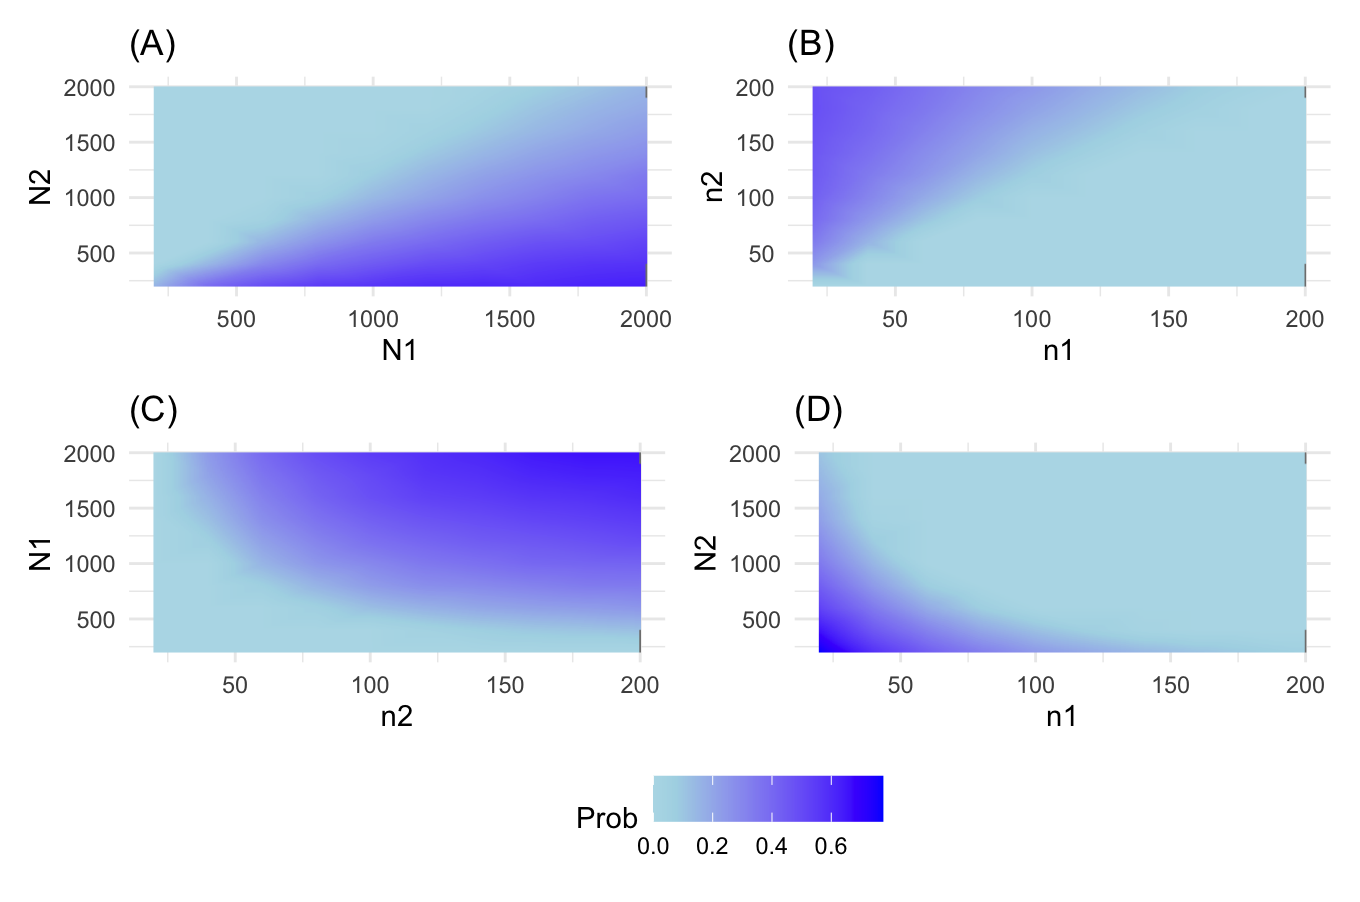
\includegraphics[width=\textwidth]{fourplot.png}
    \caption{Sensitivity Analysis for Paradox Probability}
    \label{Fig:sensitivity}
\end{figure}

Figure~\ref{Fig:sensitivity} presents the results of the sensitivity analysis for the aptitude-achievement paradox probability described in Theorem~\ref{theorem:samedistgeneral}. In Figure~\ref{Fig:sensitivity} (A), we fix $n_1 = 40$ and $n_2 = 60$, and vary $N_1$ and $N_2$ from 200 to 2000.  In Figure~\ref{Fig:sensitivity} (B), we fix $N_1 = 10^3$ and $N_2 = 10^3$, and vary $n_1$ and $n_2$ from 20 to 200. In Figure~\ref{Fig:sensitivity} (C), we fix $n_1 = 40$ and $N_2 = 10^3$, and vary $n_2$ from 20 to 200 and $N_1$ from 200 to 2000. In Figure~\ref{Fig:sensitivity} (D), we fix $N_1 = 10^3$ and $n_2 = 60$, and vary $N_2$ from 200 to 2000 and $n_1$ from 20 to 200.

As shown in Figure~\ref{Fig:sensitivity} (A), a small $N_2$ and large $N_1$ increase the paradox probability by making $\Prob\left(X_{1,(r_{1,j})} > X_{2,(r_{2,k})}\right) \to 1$. Similarly, in Figure~\ref{Fig:sensitivity} (B), a small $n_1$ combined with a large $n_2$ leads to a higher aptitude-achievement paradox probability since it drives $\Prob\left(Y_{1,(j)} < Y_{2,(k)}\right) \to 1$.


\subsection{Ratio of $N_2$ and $N_1$}

Here we investigate the effect of the ratio between $N_2$ and $N_1$ on aptitude-achievement paradox probabilities under the specifications of Corollary~\ref{corollary:samedisttop}. Let $c=\frac{N_2}{N_1}$, and vary $c$ from 0.1 to 1 in increments of 0.1. In each simulation, we fix $n_1 = 60$ and $n_2 = 40$, and vary $N_1$ from 100 to 2000. We repeat this simulation 10000 times and report the average paradox probability. 

\begin{figure}[t!]
    \centering
    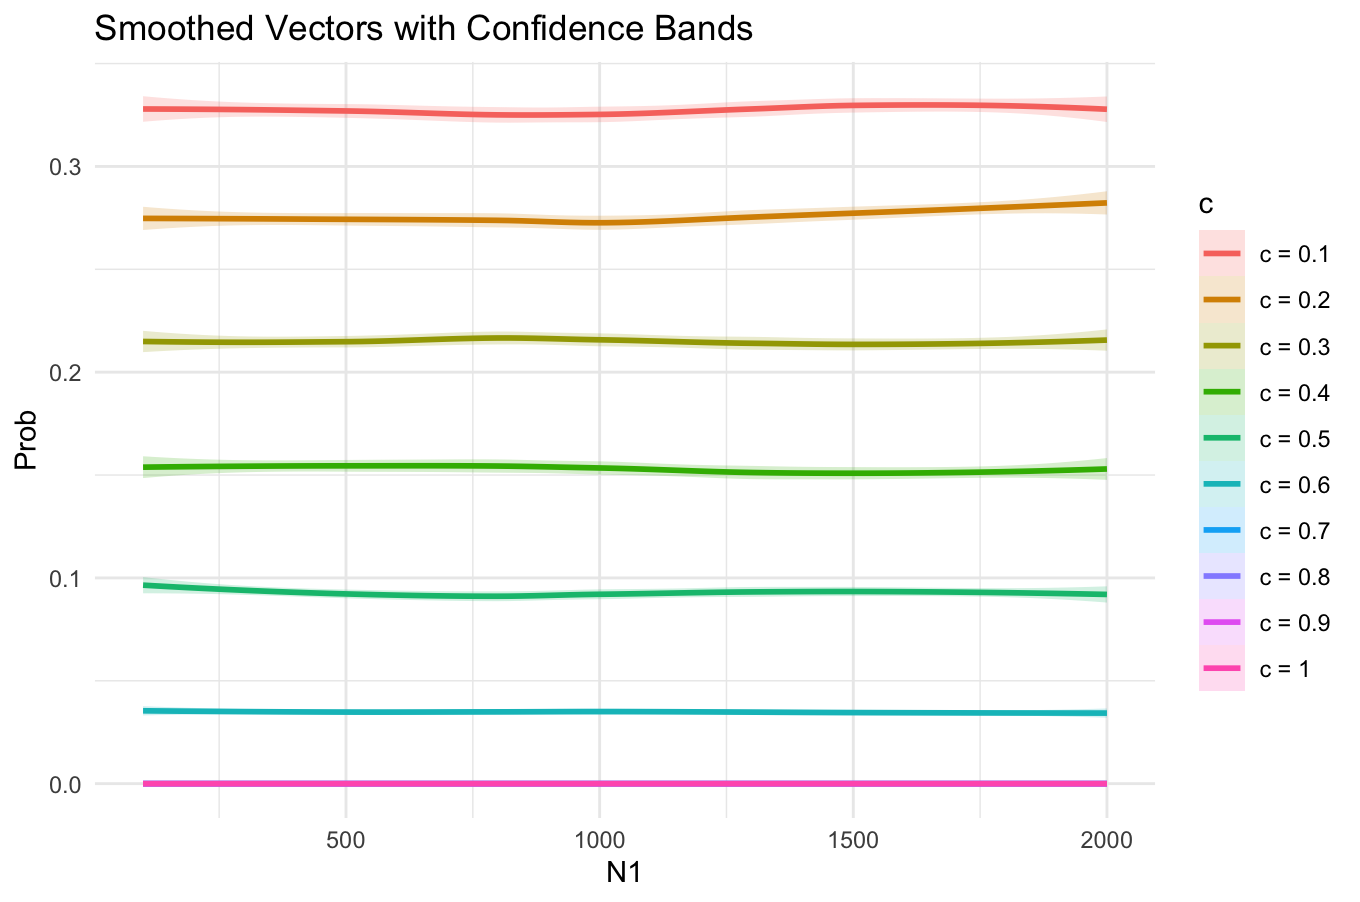
\includegraphics[width=\textwidth]{cplot.png}
    \caption{Effect of the ratio between $N_2$ and $N_1$ on aptitude-achievement paradox probabilities under the specifications of Corollary~\ref{corollary:samedisttop}.}
    \label{Fig:ratioeffect}
\end{figure}

Figure~\ref{Fig:ratioeffect} presents the results. As shown in the figure, the paradox probability decreases as $c $ increases, which is reasonable since $\Prob\left(X_{1,(r_{1,j})} > X_{2,(r_{2,k})}\right)$ decreases as $N_2 $ increases. Importantly, Figure~\ref{Fig:ratioeffect} also demonstrates that the paradox probability remains constant when the ratio between $N_2$ and $N_1$ is fixed. This implies that it is unnecessary to focus on the exact values of $N_1$ and $N_2$ when computing the paradox probability; rather, the ratio $N_2/N_1$ alone determines its value.



\subsection{Batting Averages in Major League Baseball}

We illustrate Theorem~\ref{theorem:normalgeneral} and the plug-in guarantees of Theorem~\ref{theorem:plugin} using Major League Baseball (MLB), a setting in which latent batting aptitude is indirectly observed through season-level batting averages and where both population structure and measurement environments vary substantially across eras. Figure~\ref{Fig:means-sd-full-time} displays smoothed estimates of the mean and standard deviation of batting averages for full-time players from 1871--2023.

\begin{figure}[t!]
\begin{center}
	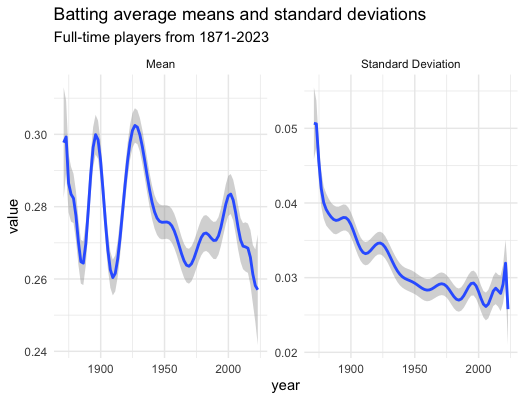
\includegraphics[scale=0.75]{means-sd-full-time.png}
\end{center}
\caption{Seasonal means and standard deviations of batting averages for full-time players from 1871--2023. Smoothing is applied to both trends.}
\label{Fig:means-sd-full-time}
\end{figure}

We treat the 2023 season as system~1 and each season from 1871--2022 as system~2. Seasonal batting averages for full-time players are modeled as Gaussian with means and standard deviations estimated via plug-in; the consistency guarantees of Theorem~\ref{theorem:plugin} therefore apply. Figure~\ref{Fig:means-sd-full-time} shows that the 2023 offensive environment exhibited both relatively low mean batting average and reduced variability compared with many historical eras. Under our specifications, we additionally have $\hat{\sigma}_1 \leq \hat{\sigma}_2$, $\hat{\mu}_1 \leq \hat{\mu}_2$, and $\frac{n_1}{N_1} \leq \frac{n_2}{N_2}$, implying that the remainder term \eqref{eq:remainder} in Theorem~\ref{theorem:normalgeneral} is negligible. Talent-pool estimates $N_i$ are taken from \citet{yan2025comparing}, which includes sensitivity analyses demonstrating robustness to reasonable perturbations of these estimates.

\begin{figure}[t!]
\begin{center}
	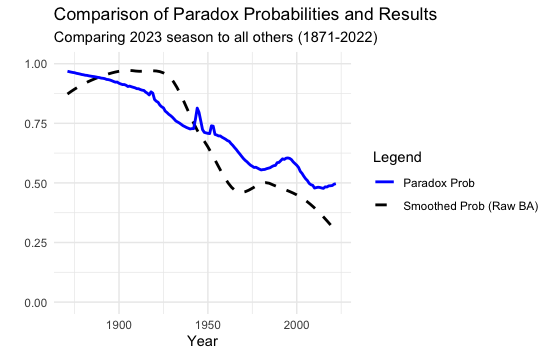
\includegraphics[scale=0.75]{paradox-prob-results.png}
\end{center}
\caption{Comparison of estimated paradox probabilities and empirical exceedance rates relative to the 2023 season, based on data from 1871--2022. The blue line shows plug-in paradox probability estimates from Theorem~\ref{theorem:normalgeneral}; the dashed black line shows a smoothed empirical exceedance rate for Luis Arraez's 2023 batting average.}
\label{Fig:paradox-prob-results}
\end{figure}

Figure~\ref{Fig:paradox-prob-results} shows that estimated paradox probabilities closely track empirical exceedance patterns across eras, indicating that the proposed framework captures structural differences in competitive depth and measurement environment rather than merely reproducing descriptive trends. In particular, the framework explains why Luis Arraez's 2023 batting average may appear modest under raw historical comparison while nevertheless corresponding to unusually high latent aptitude after accounting for population depth and contextual variation. Under Full House Modeling, Arraez's 2023 season ranks 68th all-time among full-time batters after adjustment \citep{yan2025comparing, fullhouse2025}, compared with a raw observed rank of 341. This gap illustrates how cross-context comparisons based solely on observed outcomes can induce substantial latent-observed ranking reversals, precisely the phenomenon quantified by the paradox probability.


%We now apply Theorem~\ref{theorem:normalgeneral} and the reliability guarantees in Theorem~\ref{theorem:asymptotic} to evaluate the contextual extremeness of observed outcomes in a real-world system where the underlying distribution of aptitude is not directly observable and evolves over time. Major League Baseball (MLB) offers a canonical example of such a system. Here, player skill (latent batting aptitude) is inferred only indirectly through season-level observed outcomes (batting averages), which are shaped by changing population structures and environmental variance. In particular, MLB introduced a series of rule changes in 2023 intended to increase in-game action, including a restriction on defensive positioning designed to raise batting averages on balls in play (BABIP) \citep{castrovince2023mlb}. Figure~\ref{Fig:means-sd-full-time} presents smoothed estimates of the mean and standard deviation of batting averages for full-time players from 1871 to 2023.
%\begin{figure}[t!]
%\begin{center}
%	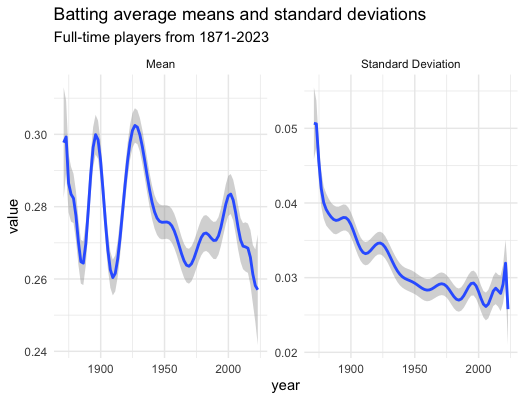
\includegraphics[scale=0.75]{means-sd-full-time.png}
%\end{center}
%\caption{Seasonal means and standard deviations of batting averages for full-time players from 1871-2023. Smoothing is applied to both trends.}
%\label{Fig:means-sd-full-time}
%\end{figure} 

%The 2023 season saw an increase in mean batting average for full-time players of 0.0057 (corresponding to an additional hit about every four baseball games) with a reduction in variability. A two-sample test for differences in batting averages among full-time players from the 2023 and 2022 seasons has a p-value of 0.039. Thus, rule changes seemed to be effective in yielding increased batting averages\footnote{Technically, \cite{castrovince2023mlb} referred to MLB's desire to increase batting averages on balls in play (BABIP) while this analysis focused on batting averages. BABIP increased by 0.0061 from 2022 to 2023.} Moreover, the 2023 MLB batting leader Luis Arraez had a 0.354 batting average which was the first batting average to exceed .350 (a mark of excellence) since Josh Hamilton in 2010. 

%We now apply Theorem~\ref{theorem:normalgeneral} to quantify paradox probabilities for extreme batting averages, treating the 2023 season as system~1 and each season from 1871 to 2022 as system~2. Seasonal batting averages of full-time players are assumed normally distributed, with means and standard deviations estimated via plug-in; the reliability guarantees of Theorem~\ref{theorem:plugin} apply. Figure~\ref{Fig:means-sd-full-time} shows that both the average and variability of batting averages in 2023 are among the lowest observed, indicating a historically suppressed environment. Moreover, with our specifications we have that $\hat{\sigma}_1 \leq \hat{\sigma}_2$, $\hat{\mu}_1 \leq \hat{\mu}_2$, and $\frac{n_1}{N_1} \leq \frac{n_2}{N_2}$, so the remainder term \eqref{eq:remainder} in Theorem~\ref{theorem:normalgeneral} is negligible. The talent pool estimates $N_i$ are taken from \cite{yan2025comparing}, which includes sensitivity analyses showing that qualitative conclusions are robust to reasonable perturbations of these estimates.

%\begin{figure}[t!]
%\begin{center}
%	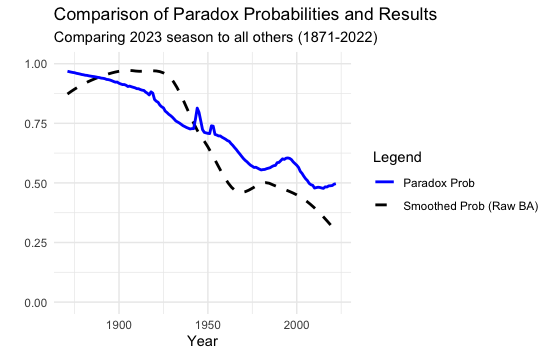
\includegraphics[scale=0.75]{paradox-prob-results.png}
%\end{center}
%\caption{Comparison of paradox probabilities and empirical exceedance rates relative to the 2023 season, based on data from 1871--2022. The blue line shows estimated paradox probabilities via plug-in using Theorem~\ref{theorem:normalgeneral}. The black dashed line displays a smoothed empirical exceedance rate for Arraez's 2023 batting average.}
%\label{Fig:paradox-prob-results}
%\end{figure}

%Importantly, the estimated paradox probabilities closely track empirical exceedance patterns across eras (Figure~\ref{Fig:paradox-prob-results}), indicating that the proposed framework captures the structural forces governing discrepancies in cross-era rankings rather than merely reproducing descriptive trends. In particular, the framework explains why certain modern performances, such as Arraez's 2023 batting average, may appear modest in raw historical comparisons while nevertheless corresponding to exceptionally high latent aptitude after accounting for differences in population depth and measurement environment. Under Full House Modeling, Arraez's 2023 season ranks 68th all-time among full-time batters after these adjustments \citep{yan2025comparing, fullhouse2025}, compared to a raw observed rank of 341. This gap illustrates how observed rankings can be systematically distorted by changes in population structure and measurement conditions, and how the paradox probability provides a formal quantitative measure of this distortion.



\section{Discussion}

The aptitude-achievement paradox arises when an individual from one context demonstrates higher latent aptitude but simultaneously lower observed achievement than an individual from another context. Although widely encountered in education, labor economics, psychometrics, medicine, and sports analytics, measuring the frequency of this paradox under realistic data-generating regimes is nontrivial. In this article, we formalize Full House Modeling and investigate the probabilities of observing paradoxes between latent aptitude and observed achievement in comparative analysis of individuals across contexts.

%Full House Modeling formalizes the comparison of individuals' performance across distinct contexts based on the large source population size $N$, thereby offering a more nuanced understanding of individual differences and the impact of contextual factors on observed outcomes. In parallel, the causal bootstrap \citep{imbens2018causal} highlights that valid causal inference similarly requires situating the observed sample within large source population to properly account for sampling uncertainty. By comparison, the Rasch model \citep{bond2013applying} ensures that comparisons of individuals' abilities are independent of the specific items administered, and that comparisons of item difficulties are independent of the sample of individuals tested, but it does not explicitly leverage the source population structure. Likewise, Bayesian hierarchical modeling \citep{BRL99} with the application in comparison of individuals' latent aptitudes typically captures population-level variation through seasonal or group-level random effects rather than through an explicit embedding into a large source population. 

This work is a theoretical clarification of Full House Modeling and provides the definition and solutions for an inferential target, the aptitude-achievement paradox, which extend beyond the baseball motivations in \cite{yan2025comparing}. In doing so, we note the baseball origins of this work, as articulated by Stephen Jay Gould in his 1996 book \emph{Full House: The Spread of Excellence from Plato to Darwin} (p. 122), from which this framework takes its name: ``Baseball is a truly remarkable system for statisticians, manifesting two properties devoutly to be wished, but not often encountered, in actual data: an institution that has worked by the same rules for a century, and has compiled complete data (nothing major missing) on all measurable aspects of its history.'' In this way, baseball, with its century of consistent rules and comprehensive measurement, served as an ideal proving ground for the Full House framework  \citep{yan2025comparing}. Gould's discussion emphasized the possibility that population structure and selection may substantially influence observed achievement distributions across eras. The present work formalizes one probabilistic framework through which such effects can be quantified and analyzed.

We derive closed-form expressions for paradox probabilities under Full House data generating models in two regimes: (i) when observed achievements are i.i.d., and (ii) when context-specific summaries are independent normals with distinct means and variances. The probability rises with population-size asymmetry (large $N_1$, small $N_2$) and sampling asymmetry (small $n_1$, large $n_2$). Moreover, for a fixed population-size ratio $N_2/N_1$, it is unchanged by proportional rescaling of the sample sizes $(n_1,n_2)$. We also develop bounds for more general settings and show that, when observed achievement is normal, plug-in estimators yield reliable paradox-probability estimates.

The present analysis focuses on rank-preserving structural couplings and highly selective observation regimes, particularly top-$n$ selection mechanisms. Extending the framework to settings involving stochastic measurement error, imperfect ranking preservation, probabilistic selection, or heterogeneous latent aptitude distributions remains an important direction for future work. Likewise, while the present paper studies pairwise paradox probabilities, broader ranking-level functionals may also be of interest.

Beyond baseball, the aptitude-achievement paradox has potential implications for educational evaluation and admissions. When students are compared across institutions of differing selectivity, observed performance metrics may systematically misrepresent underlying aptitude due to differences in competition depth, selection mechanisms, and measurement environments. The methodology developed here provides a formal way to quantify such latent-observed reversals under explicit assumptions on selection and measurement processes. More broadly, the framework highlights how cross-context comparisons based solely on observed outcomes can become sensitive to differences in population structure, selection intensity, and measurement environment.

%By elevating aptitude-achievement paradoxes from an anecdotal concern to a model-based, estimable quantity, our framework clarifies when cross-context comparisons are trustworthy, when they are fragile, and how to report that fragility responsibly. This closes the loop between principled latent measurement, realistic selection processes, and interpretable comparative claims.
By formalizing aptitude-achievement reversals as an estimable probabilistic quantity, this work provides a framework for studying how population depth, selective observation, and measurement structure jointly shape cross-context comparisons. More broadly, the results illustrate how latent-observed ranking reversals can arise systematically under heterogeneous selection and measurement regimes.


\section*{Acknowledgements}

We are grateful to G\"ok\c{c}e Dayan\i kl\i, Karl Oskar Ekvall, Eren C K\i z\i lda\u{g}, Jingbo Liu, Susu Zhang and many others for helpful comments, great discussions, and inspiration. We acknowledge the use of ChatGPT and Claude to aid with proofreading and writing clarity. 


\section*{Supplementary Materials}

The Supplementary Materials contain proofs of mathematical results, together with auxiliary Monte Carlo simulations provided solely for numerical intuition for Theorem~\ref{theorem:normalgeneral}.


\bibliography{FHM.bib}
\bibliographystyle{plainnat}




\end{document}





